\section{Replications}
 
\subsection{Design}

For the purpose of this study, we choose five prominent studies from the broad field of international relations and international political economy that utilize relation data \citep{mcdonald:2004, reiter:stam:2003, rose:2004, weeks:2012, gibler:2017}. We chose to replicate studies that were written fairly recently, since 2000, and that have been cited over 100 times. Each of these pieces was published in a prominent journal and is well-known in the literature. They all used the standard approach in political science, which is to employ some form of general linearized regression that ignores dyadic interdependencies. Post estimation, standard errors are often adjusted in an attempt to account for clustering of observations.

\begin{table}
\caption{Features of the Studies Replicated. }
	\begin{tabular}{lcccccc}
		 & Model & \# of Actors & Years  & \# of Dyads & Type of Dyads & Clustered $\sigma_{\hat{\beta}}$ \\ \hline\hline
		Weeks (2012) & Logit & & & $901,540$ & Directed & Robust \\
		Reiter \& Stam (2003) & Logit & & & $753,456$ & Directed & Robust \\
		McDonald (2004) & Logit & & & $92,354$ & Undirected & Robust\\		
		Gibler (2017) & Logit & & & $650,557$ & UnDirected & no \\		
		Rose (2004) & OLS & & & $234,597$ & Directed & Robust \\
	\hline\hline
	\end{tabular}
\end{table}

We obtained the data for each of these studies from their replication archives and replicated the main results of each of the articles.\footnote{Without exception this was straightforward to accomplish, thanks to an increasing norm in the social sciences of open data sharing.} We examine each of the models using the AME framework described above.  Our goal is to ascertain whether the ignored interdependencies---the non-iid structure of the relational data---would result in different model estimates when they were addressed in an AME framework, and more importantly to see if there were substantive opportunities that were presented with the dynamic factor approach.  

Finally, we assess whether there is any substantive finding that emerges or indeed if any disappear once the interdependencies in the data are modeled.

The broader goal, beyond introducing the use of the AME framework in an applied setting, is to examine the extent to which interdependencies within typical dyadic data make much difference in what we have learned about international relations from empirical studies over the past decade or so.  We believe that it does, and that the dynamic latent factor model provides a step forward.

\begin{table}[ht]
\centering
	\begin{tabular}{l| p{7cm} l}
	& \multirow{2}{*}{Central Finding} & Does it Replicate \\ 
	& &  in a Network Model? \\
	\hline\hline
		Weeks (2012) & Bosses, Juntas and Strongmen are more Aggressive, Machines are Not & \textbf{Fails to Replicate} \\
		\hline
		Reiter \& Stam (2003) & Personalist Regimes Attack Democracies, Not Vice Versa & Replicates \\ 
		\hline
		McDonald (2004) & Lower Trade Barriers and Higher Trade Lead to Peace & \textbf{Fails to Replicate} \\ 
		\hline
		Gibler (2017) & Power Parity at time of Entry to International System Inceases Conflict & \textbf{Fails to Replicate} \\ 		
		\hline
		Rose (2004) & WTO Membership Does not Effect Trade & Replicates \\ 
	\hline\hline
	\end{tabular}
	\caption{Here we provide a brief summary of the key variable in each of the five replications and a note about whether or not the finding is replicated when using our network based approach. Cases in which the finding is not replicated are highlighted in bold.}
	\label{tab:modelFindingSumm}
\end{table}

We also examine the accuracy of the predictions made with each approach. Out of sample cross validation strategy. 

% % % % % % % % % % % % % % % % % % 
By accounting for exogenous and network dependent patterns that give rise to conflict systems we are able to better account for the data generating process underlying relational data structures. To show that this is the case, we examine whether our approach achieves better predictive performance in an out of sample context than traditional dyadic models. To evaluate our model, we randomly divide the $\binom n 2 \times T$ data values into $k=30$ sets, letting $s_{ij,t}$ be the set to which pair $ij,t$ is assigned. Then for each $s \in \{1,\ldots,k\}$, we:

\begin{enumerate}
	\item estimate model parameters with $\{y_{ij,t}: s_{ij,t} \neq s\}$, the data not in set $s$,
	\item and predict $\{\hat{y}_{ij,t}: s_{ij,t} = s\}$ from these estimated parameters. 
\end{enumerate}

\noindent The result of this procedure is a set of sociomatrices $\bm \hat Y$, in which each entry $\hat y_{ij,t}$ is a predicted value obtained from using a subset of the data that does not include $y_{ij,t}$. 

We set a number of benchmarks for comparison. First we compare the AME model to a GLM model using the same covariates to show the effect of accounting for network dependencies on predicting conflict. We supplement this with an alternative GLM that includes not just these covariates, but also a lagged dependent variable and a lagged reciprocity term. The lagged dependent variable is the equivalent of saying that conflict and peace are relatively likely to persist between dyads, while the inclusion of a lagged reciprocity term in a GLM framework is a simple way to account for retaliatory strikes.

We utilize three performance criterions to compare the models: Receiver Operator Characteristic (ROC) curves, Precision Recall (PR) curves, and separation plots. ROC curves look at the trade-off between true positive rates and false positive rates at different thresholds of classification. An issue with an ROC Curve when looking at conflict, is that it is relatively rare at the dyadic level: in most years only 3\% of possible dyads are in conflict with one another. If peace is common, even a poor model will have a very low False Positive Rate. 

To better assess which models predict the presence of conflict, not just its absence, we look at PR Curves. These examine the trade-offs between the percentage of conflicts a model predicts, and the percentage of predicted conflicts which occur. Lastly, we examine separation plots \citep{greenhill:etal:2011}. These provide an intuitive visualization of the accuracy of our predictions by juxtaposing a line showing the predicted probability of conflict with whether conflict actually occurs for all cases (where the cases are sorted by the predicted probability and then colored to indicate the outcome). Here a perfect model would have all cases where conflict actually exists on the right with a predicted probability of $1$, and would predict $0$ in all other cases. All of the models' performance out of sample by these metrics are displayed in figure \ref{fig:roc_ame}. The AME model with covariates is the best performing model out of sample in all cases. This model outperforms each of the GLM variants by a notable margin.
% % % % % % % % % % % % % % % % % % 

\begin{table}[ht]
\centering
	\begin{tabular}{l|l cc}
	~ & ~ & GLM & AME \\
	\hline\hline
		\multirow{2}{*}{Weeks (2012)} & Area Under ROC Curve (AUC-ROC) & 0.64 & \textbf{0.97} \\
		~ & Area Under PR Curve (AUC-PR) & 0.00 & \textbf{0.15} \\
		\hline
		\multirow{2}{*}{Reiter \& Stam (2003)} & AUC (ROC) & 0.92 & \textbf{0.96} \\
		~ & AUC (PR) & 0.08 & \textbf{0.15} \\
		\hline
		\multirow{2}{*}{McDonald (2004)} & AUC (ROC) & 0.92 & \textbf{0.99} \\
		~ & AUC (PR) & 0.13 & \textbf{0.28} \\
		\hline
		\multirow{2}{*}{Gibler (2017)} & AUC (ROC) & 0.52 & \textbf{0.91} \\
		~ & AUC (PR) & 0.00 & \textbf{0.08} \\
		\hline
		\multirow{2}{*}{Rose (2004)} & Root Mean Squared Error (RMSE) & 3.23 & \textbf{1.99} \\
		~ & Root Median Squared Error (RMDSE) & 2.01 & \textbf{1.06} \\
	\hline\hline
	\end{tabular}
	\caption{Here we provide a summary of the out-of-sample performance based on our cross-validation strategy for each of the five replications when using the standard dyadic approach and our network based approach. Four of the five studies involved a binary dependent variable, so for those measures we provide area under the curve (AUC) statistics. The fifth involved a gaussian dependent variable and for that we use the root mean squared error (RMSE) and root median squared error (RMDSE). Cases in which our network based approach outperformed the standard approach are highlighted in bold.}
	\label{tab:modelPerfSumm}
\end{table}
\FloatBarrier

\subsection{Replication of Weeks (2012)}

\citet{weeks:2012} examines the influence of domestic institutions on the initiation of military conflicts by autocratic leaders.  She argues that in some circumstances autocrats are held accountable for their foreign policy decisions. She adds the nuance that autocratic audiences are not homogeneous. When the autocratic regime is nonmilitary, the domestic audience do not favor military actions, but in military autocracies this is not the case. Further she argues that in personalistic regimes without a military or civilian domestic audience, the leaders tend to be more likely to employ military force in their foreign policy.  To study this question, she uses a dyadic design in which the dependent variable is ``whether country A in a directed dyad initiated military conflict against country B during year t'' (page 337).  These data come from the Militarized Interstate Disputes database \citep{maoz:2005}.  One major innovation in her study resides in the nuanced way in which she conceptualized and coded regime type into four types: a) Machine, b) Junta, c) Boss, and d) Strongmen. She also includes a variety of putative control variables focusing on capabilities for both sides of the dyad, alliances, geography, trade dependence, regime instability, and the regime type of ``side B.''  She uses a logistic regression, but follows \citet{beck:etal:1998} and includes splines to capture temporal covariation in the dependent variable along with  fixed, unit effects. The analysis is done for dyads, but is considered to be from the perspective of the actor that initiated the dispute. Her time frame is from 1946-1999.  The basic finding is that a) juntas, bosses, and strongmen are more likely to initiate conflict than machines (and maybe democracies) and that b) machines are no more belligerent than democracies.  These insights are mainly determined by looking at coefficients and their putative significance in Tables 1 and 2 (pages 339--340). She makes the argument that ignoring important nuances between different types of autocracies hinders our understanding of the initiation of military conflict by autocracies. 

The replication of \citet{weeks:2012} likely has the sharpest divergence between the General Linear Model results and those of the AME Model. In Weeks's initial models, as detailed in figure \ref{fig:weeksCoef} she finds that machines are less prone to initiate conflict than the reference category, whereas Juntas, Bosses and Strong-men are more conflict-prone, in line with her theoretical expectations. When we look at the posterior distribution of these coefficients in the AME results, we find that none of these values are distinguishable from zero. We similarly find less pronounced effects for military capabilities. One explanation for this divergence is the AME model's ability to account for third order effects. Inspection of the multiplicative effects in figure \ref{fig:weekscirc} reveals a number of clusters of states which exhibit structural equivalence -- in the top right corner we see states like the US, the UK, and Israel who often send conflict to similar targets. In particular, we observe a cluster of ``rogue states,'' who are receivers of conflict, in the top right (Iran, Iraq, Syria, Libya, North Korea). In the bottom corner we see a cluster of authoritarian senders including Iraq, Russia, Syria, North Korea and China. In general, these clusters have similar governmental types (Iraq, Syria, Libya, and North Korea all fell under the ``boss" category), and similar conflict behavior. So, in the GLM, which ignores these third order dependencies, much of these results might have been attributed to regime type. The AME model, on the other hand, finds that it is more efficient to attribute this behavior to the multiplicative effects. In terms of out of sample performance, shown in figure \ref{fig:weeksauc}, the AME model performs markedly better than the GLM out of sample, lending credence to the possibility that these third order dependencies cause spurious effects for regime type.

\begin{figure}
	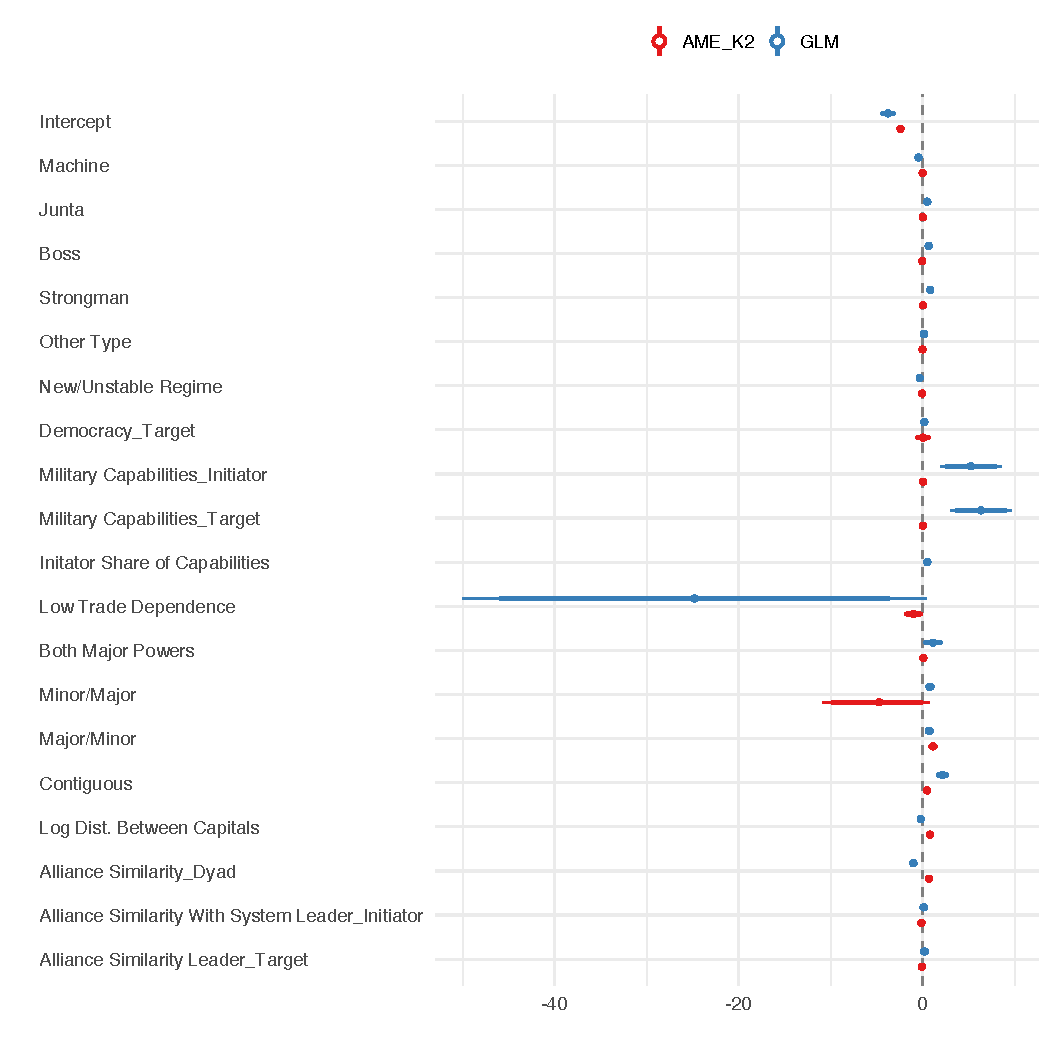
\includegraphics[width=\textwidth]{weeks_coefs_all.pdf}
	\caption{\label{fig:weeksCoef} Coefficient plot of Weeks' (2012) original model (blue) compared to AME model (red). }
\end{figure}

\begin{figure}
\centering   
	\subfigure[AUC]{\label{fig:weeksauc}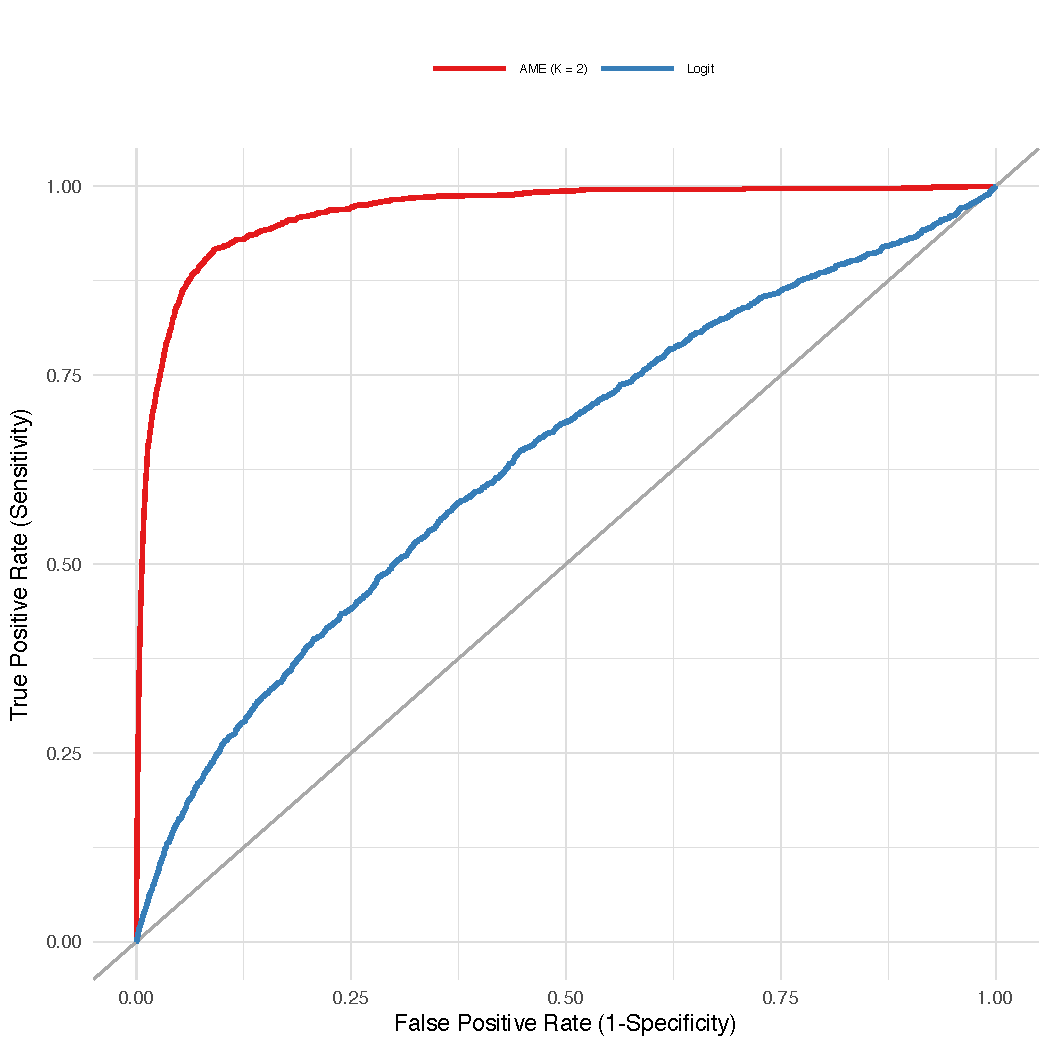
\includegraphics[width=65mm]{weeks_auc_outsamp.pdf}}
	\subfigure[Precision and Recall]{\label{fig:reitpr}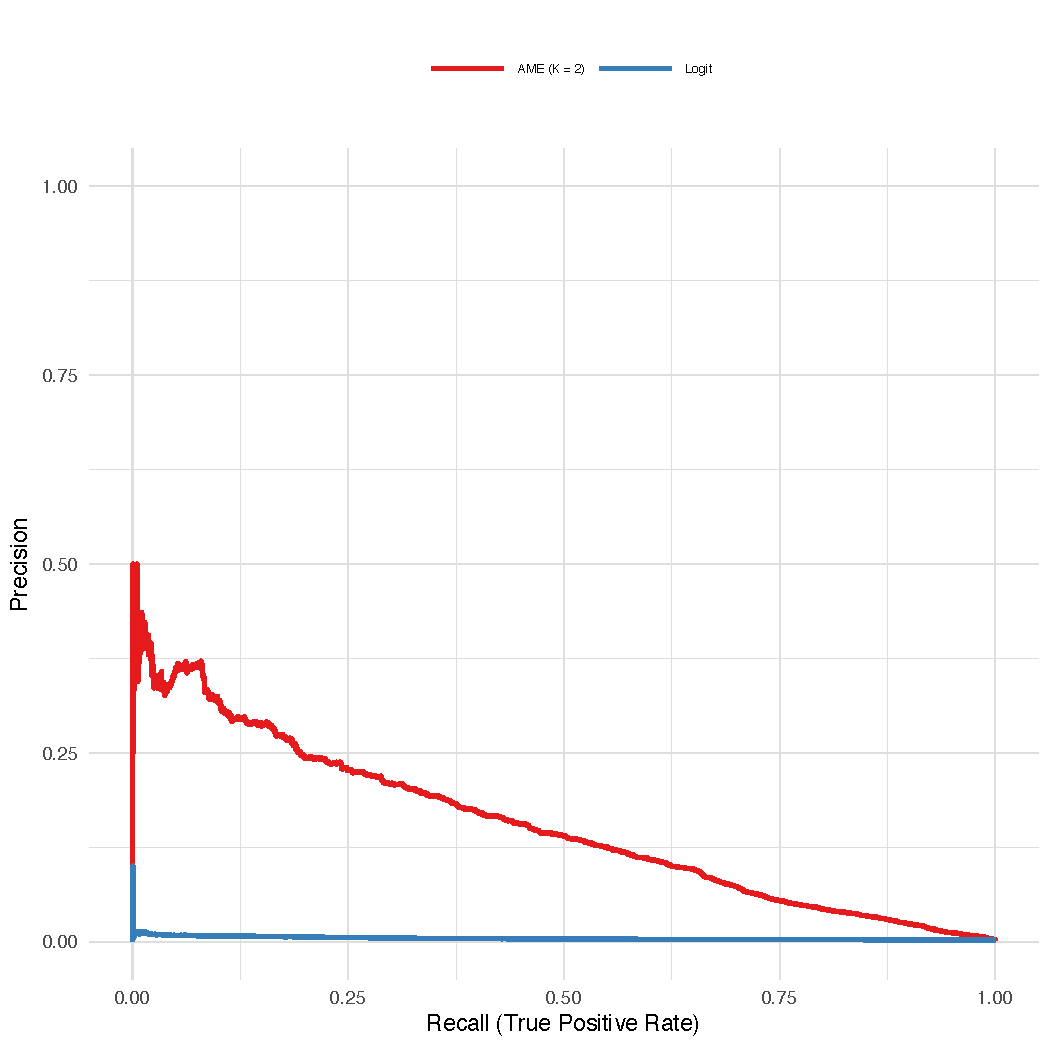
\includegraphics[width=65mm]{weeks_pr_outsamp.pdf}}
	\caption{Assessments of out-of-sample predictive performance for Weeks (2012) using ROC curves and PR curves.}
\end{figure}

\begin{figure}
	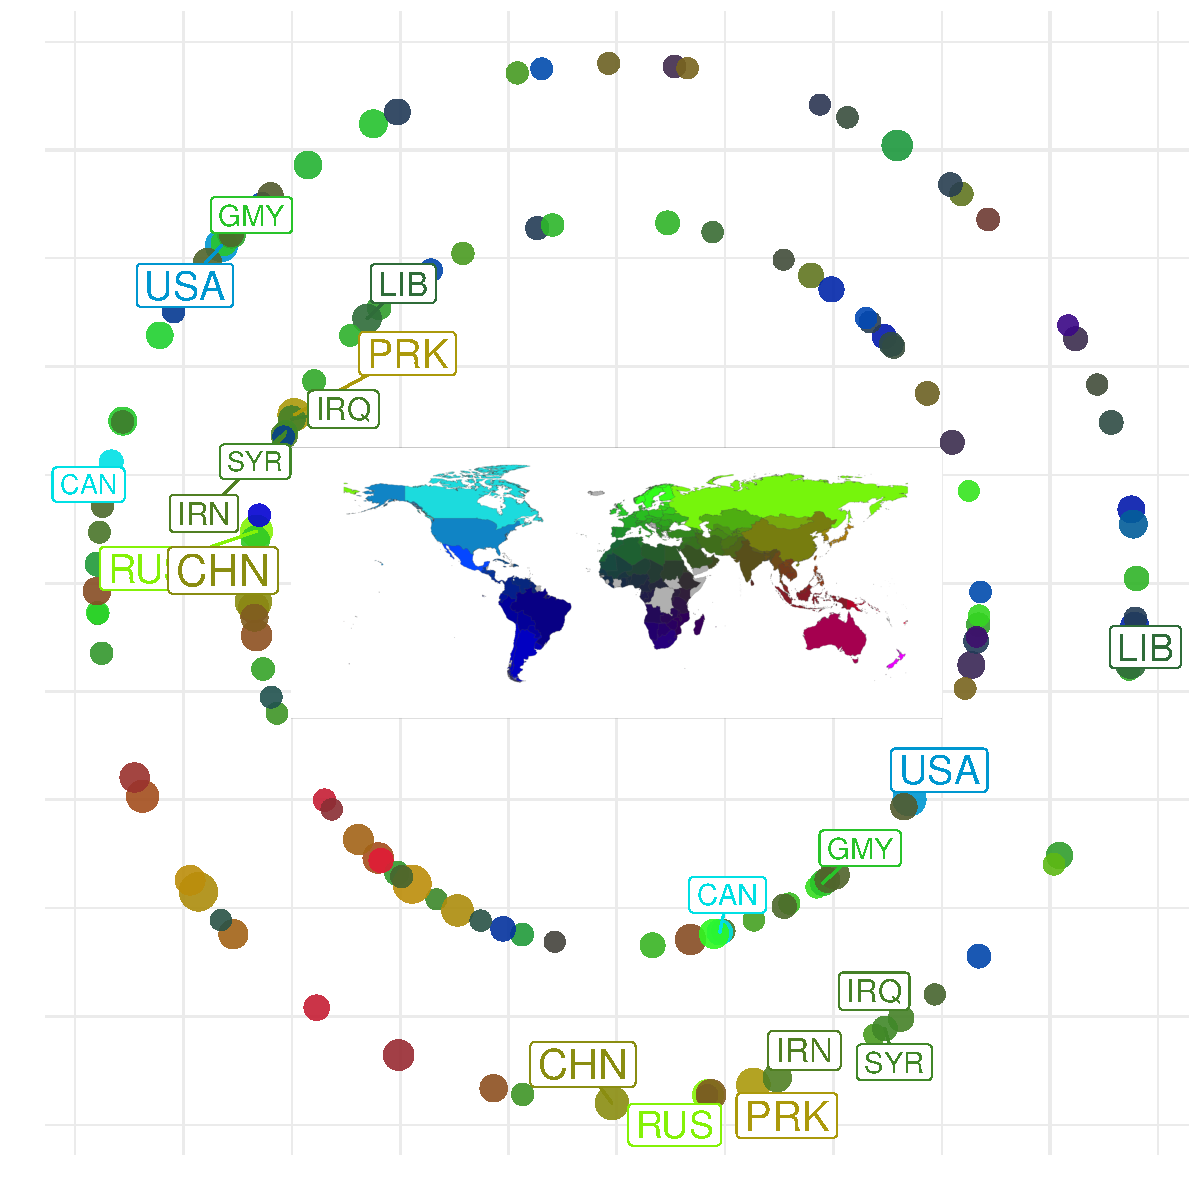
\includegraphics[width=\textwidth]{weeks_circPlot.pdf}
	\caption{\label{fig:weekscirc} Visualization of multiplicative effects for Weeks (2012). Blue represents groups with common sending patterns and red represents groups with common receiving patterns.}
\end{figure}

\subsection{Replication of Reiter \& Stam (2003)}

\citet{reiter:stam:2003} examine the relationship between democracy, dictatorship and the initiation of militarized disputes.  They use directed dyads and find that dyads involving a democratic leader on the one hand and a personalist dictator on the other tend to be violent. They also discover that dictators are likely to challenge democracies, but that this is not reciprocal.  In addition, military regimes and single-party regimes are more prone to initiate disputes with democracies, than the other way around.  They use the MID data, but note that ``We code a state as having initiated a dispute if it is on `side A' of a MID, the conventional approach to coding initiation. This means that the state was on the side that took the first action in the dispute, whether that action was the threat, display, or use of force. We code joiners as initiators or targets, though the results do not change if we do not code joiners as initiators or targets. \ldots Though coding initiation will always be difficult, the `side A' variable has been widely used in past conflict scholarship (page 334).'' Independent variables are largely taken from an earlier study and focus on various encodings of regime types, contiguity, alliance, and capability measures. As is prevalent in these kinds of studies, Reiter \& Stam employ a logistic regression that includes an indicator of the time since the last dispute as well as three cubic splines. The database for this study is constructed using EUGene \citep{bennett:stam:2000} and comprises approximately three-quarters of a million stacked dyads. Based on their statistical analysis, they conclude that institutional constraints affect the propensity of democratic and non-democratic leaders to engage in military conflict. 

In the original model, the variable ``Pers/Democ Directed Dyad" (which represents a Personalist $\rightarrow$ Democractic directed dyad) is clearly positive while the variable ``Democ/Personalist Directed Dyad'' is zero and the difference between the two coefficients is clearly distinct from zero. In our replication using the AME framework, we also find that Pers-Democ directed dyad has a positive effect with zero excluded from the 95\% confidence interval while Democ-Pers directed dyad is indistinguishable from zero. Using this model, however, we can no longer conclusively say that the Pers/Democratic coefficient is larger than the Democ/Personalist one.
Our replication using the AME approach therefore cast doubt on Reiter \& Stam's key claim that MIDs initiated by personalist dictatorships against democracies are more likely than MIDS initiated by democracies. Further, the effect of most of the covariates in the literature thought to predict interstate MIDs are much closer to zero when using the AME framework, as seen in Figure~\ref{fig:reitCoef}. Finally, our modeling approach outperforms the original model by better, and more accurately, predicting MIDs out-of-sample (Figure~\ref{fig:reitauc} and Figure ~\ref{fig:reitpr}).  

\begin{figure}
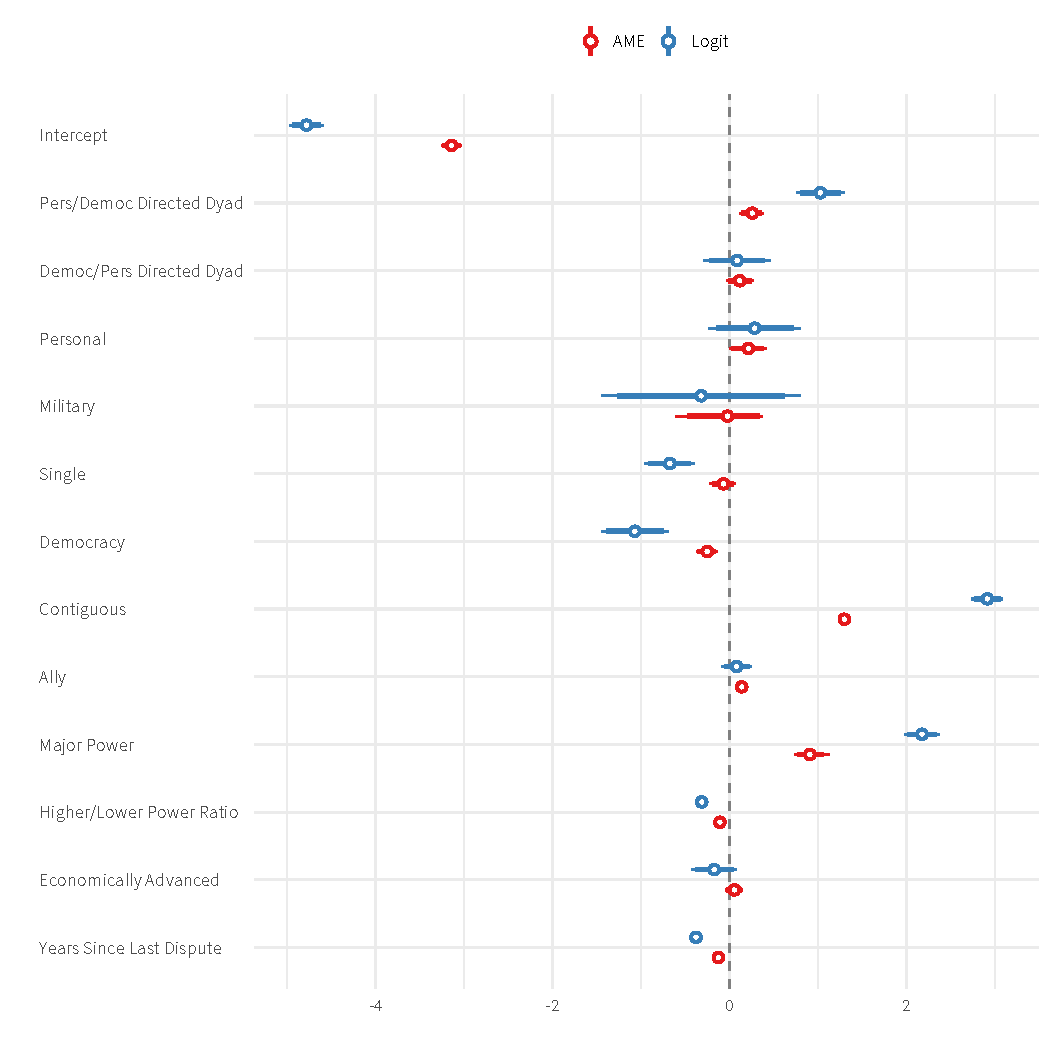
\includegraphics[width=\textwidth]{reiter_coefs_all.pdf}
\caption{\label{fig:reitCoef} Coefficient plot of Reiter \& Stam (2003)'s original model (blue) compared to AME model (red). }
\end{figure}

\begin{figure}
\centering   
\subfigure[AUC]{\label{fig:reitauc}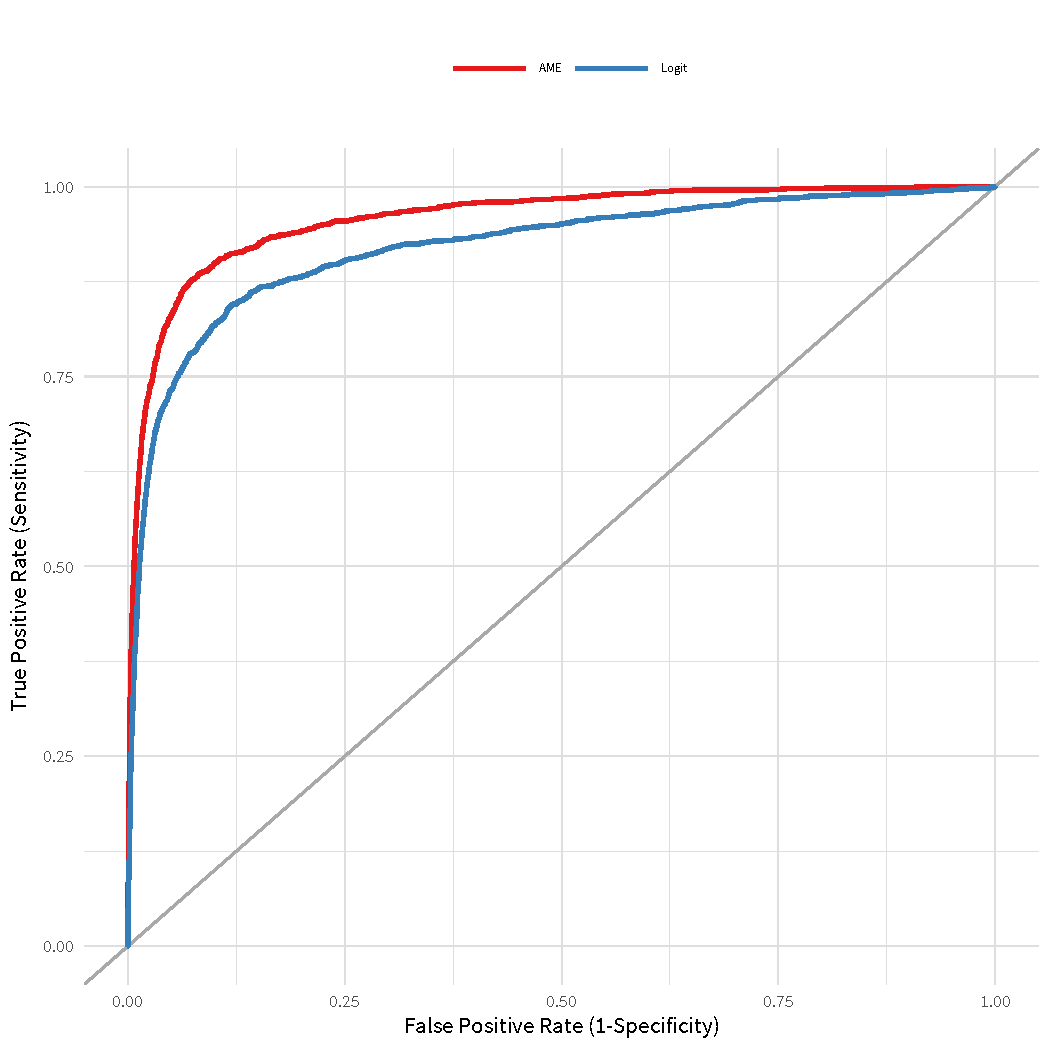
\includegraphics[width=65mm]{reiter_auc_outsamp.pdf}}
\subfigure[Precision and Recall]{\label{fig:reitpr}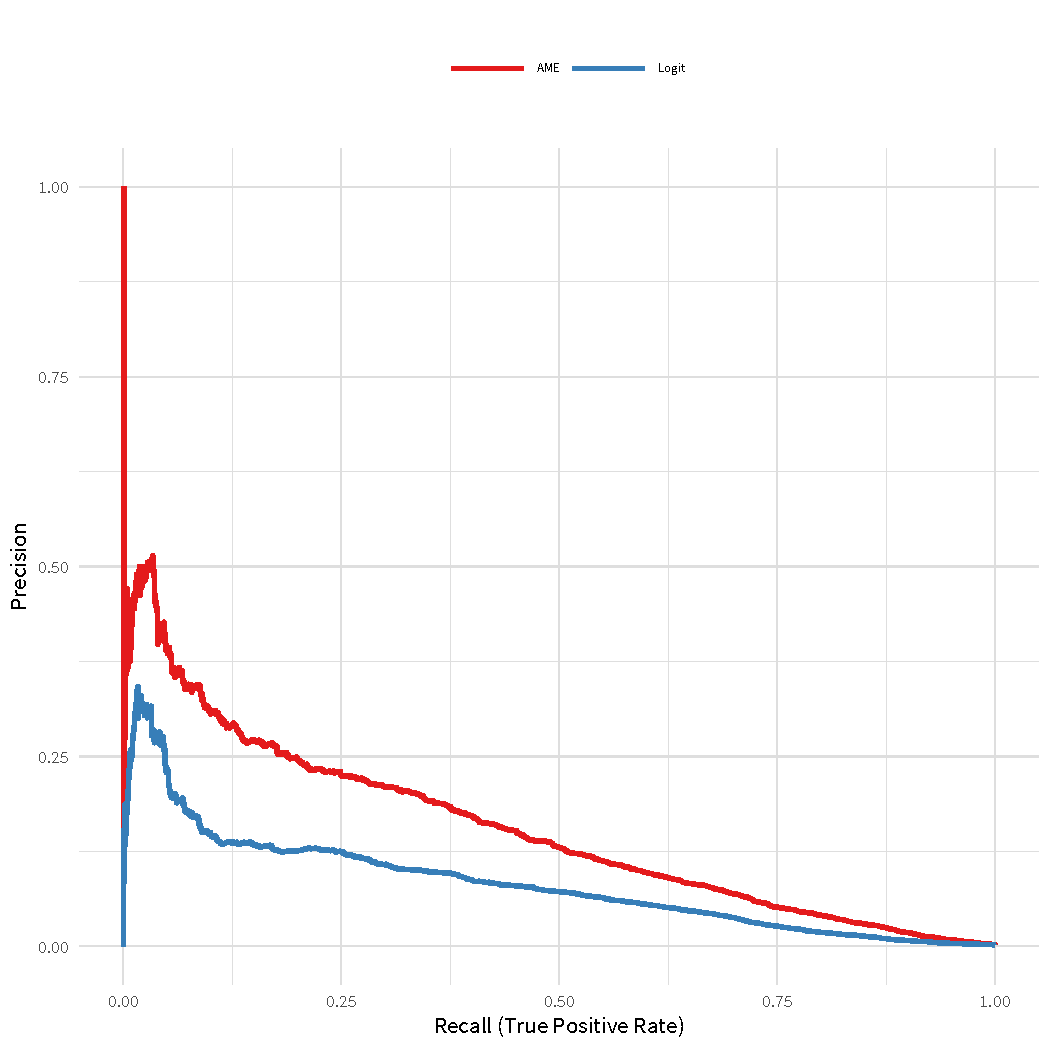
\includegraphics[width=65mm]{reiter_pr_outsamp.pdf}}
\caption{Assessments of out-of-sample predictive performance for Reiter \& Stam (2003) using ROC curves and PR curves.}
\end{figure}

\newpage
\subsection{Replication of Rose (2004)}

In 2004, Andrew Rose published a study in the \textit{American Economic Review} \nocite{rose:2004} that proved to be quite controversial in terms of macroeconomic trade theory and in terms of trade policy in a variety of nations. It also provoked a number of responses in the international political economy literature \cite{tomz:etal:2007,ward:etal:2013}.  Rose's basic argument is that despite longstanding arguments made by trade theorists and the World Trade Organization that WTO membership fosters greater cooperation and thereby more trade among its members, the empirics do not bear out such claims. He uses a standard gravity model with dyadic data on bilateral merchandise trade (not services) for $175$ countries over a period of five decades. Estimating this model using OLS within many differing contexts, his conclusion was that: ``An extensive search reveals little evidence that countries joining or belonging to the GATT/WTO have different trade patters from outsiders... (2004, page 98, abstract).''  The data for this study have been widely used in replications by many searching for the missing effects of the WTO---as well as preferential trade agreements, bilateral investment theories, and other aspects of modern trade theory.  

When we compare the results of Rose's original OLS model to our model that accounts for network dependencies, the results are generally similar. As you can see in Figure~\ref{fig:roseCoef}, the main result of the model -- the null effect of membership in the WTO, as represented by the ``One-In" and ``Both-In" variables -- remains when we move from an OLS to a Gaussian AME model. The most striking difference between the models is that, while in the original model there was a clear positive relationship between Real GDP and Trade, most of this effect vanishes in the AME model. The random effects shown in Figure~\ref{fig:roser} reveal the cause of much of this divergence. Here, the states with the most positive random effects are also states with high GDP, though not necessarily high GDP/capita.\footnote{Note: Qatar exhibits strongly negative random effects.} Thus, the effect of GDP in the original model was, in part, an artifact of first-order dependencies. Most of the other results of the model are constant across each model, though some geographic features, such as islands and landlocked states, have a more clear effect on trade once we account for these network dependencies. Excitingly, when we account for network interdependencies, we observe a markedly lower Root Mean Squared Error out of sample -- 3.23 for the OLS model and 1.77 for the AME model.

\begin{figure}
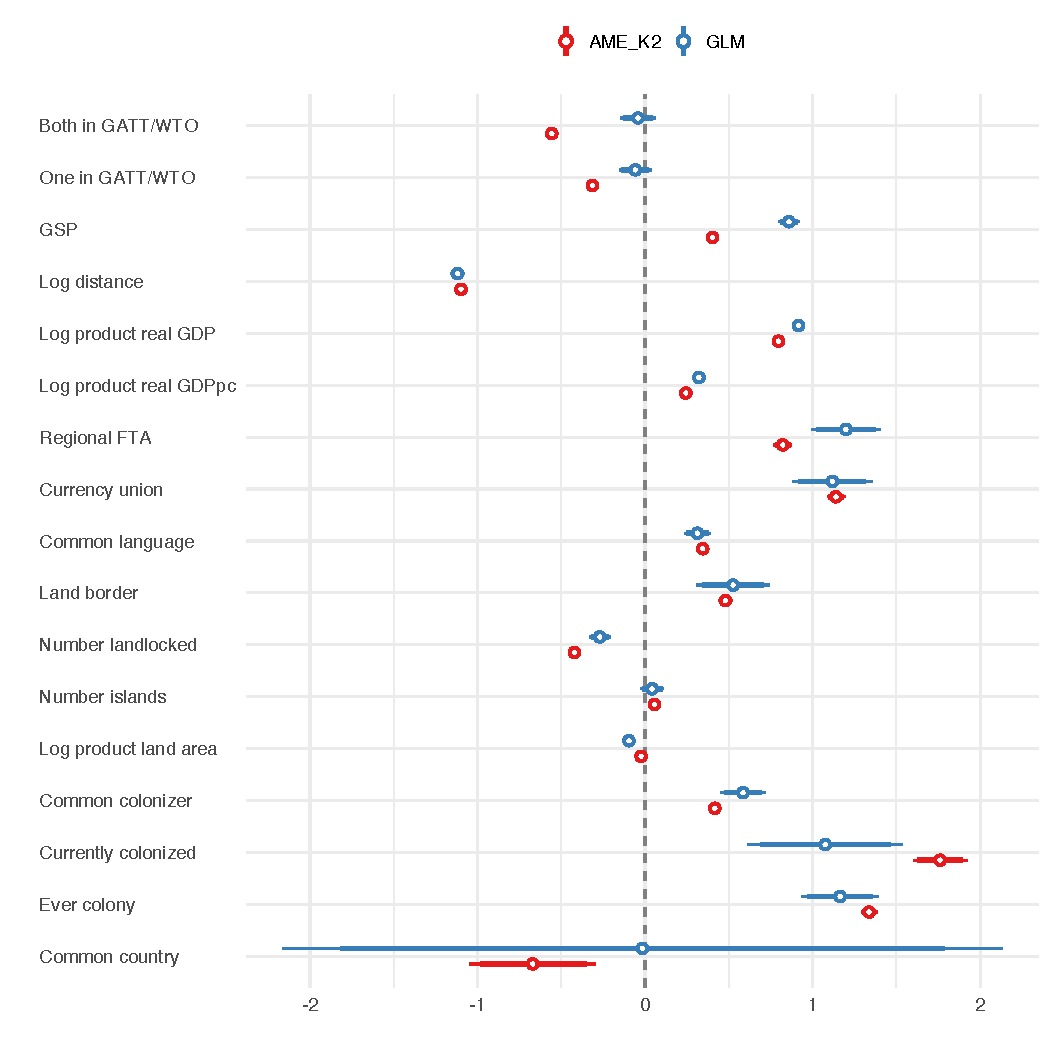
\includegraphics[width=\textwidth]{rose_coefs_all_final.pdf}
 \caption{Coefficient plot of Rose (2004)'s original model (blue) compared to AME model (red).}\label{fig:roseCoef}
\end{figure}


\begin{figure}
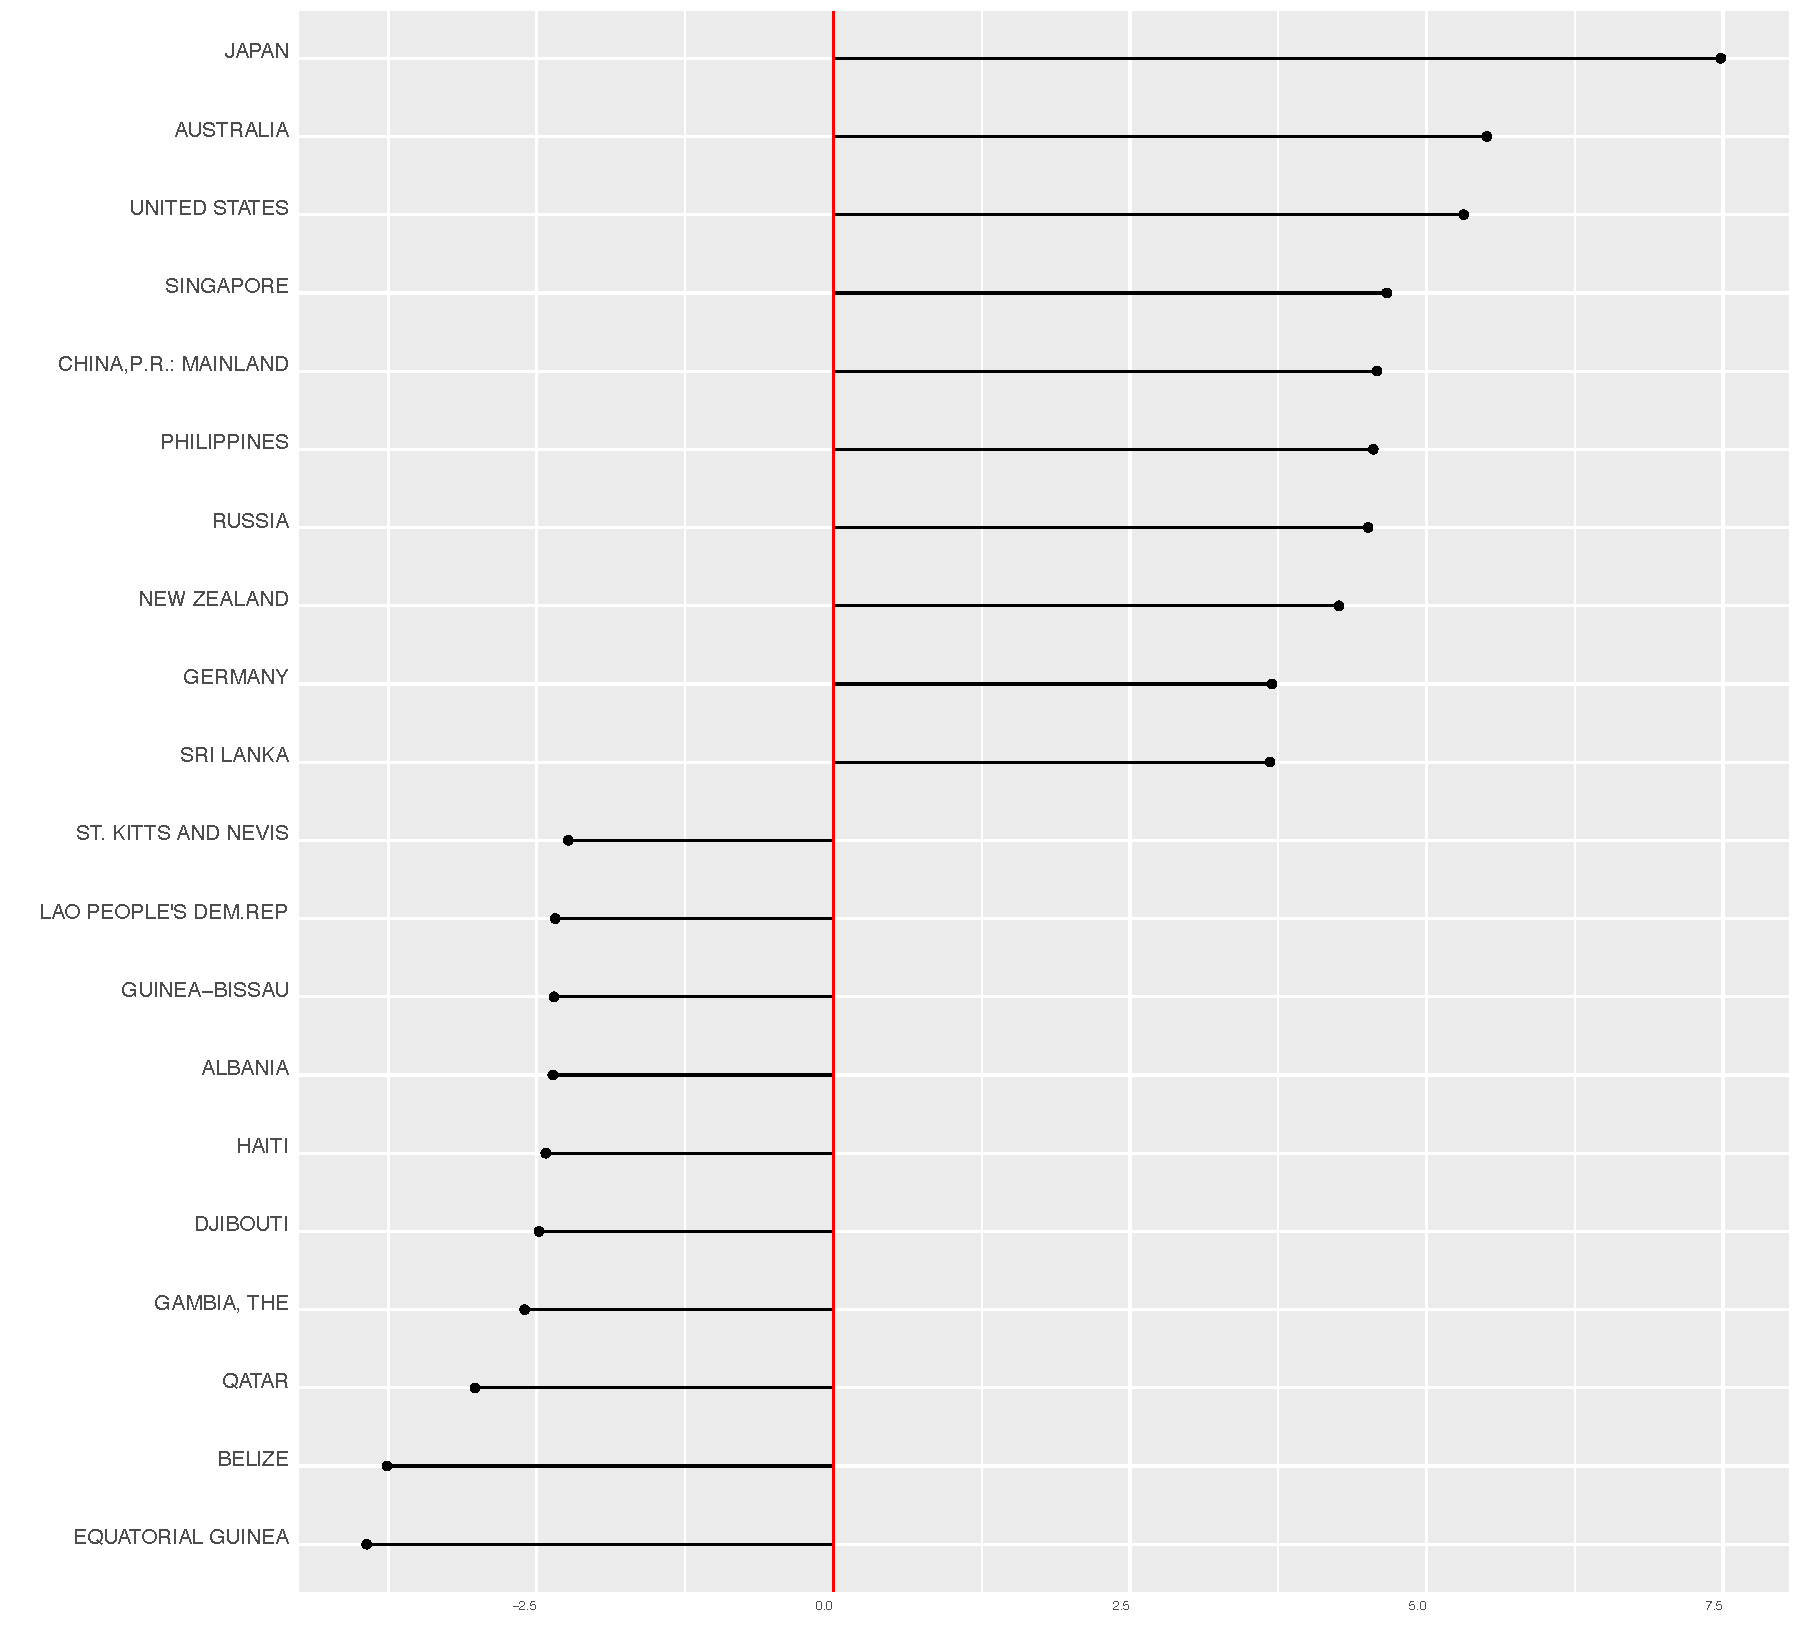
\includegraphics[width=\textwidth]{ABplot_rose_top10.pdf}
 \caption{Nodal Random Effects for AME estimation of Rose (2004).}\label{fig:roser}
\end{figure}

%\begin{figure}
%\centering   
%\subfigure[Nodal Random Effects]%{\label{fig:rosesend}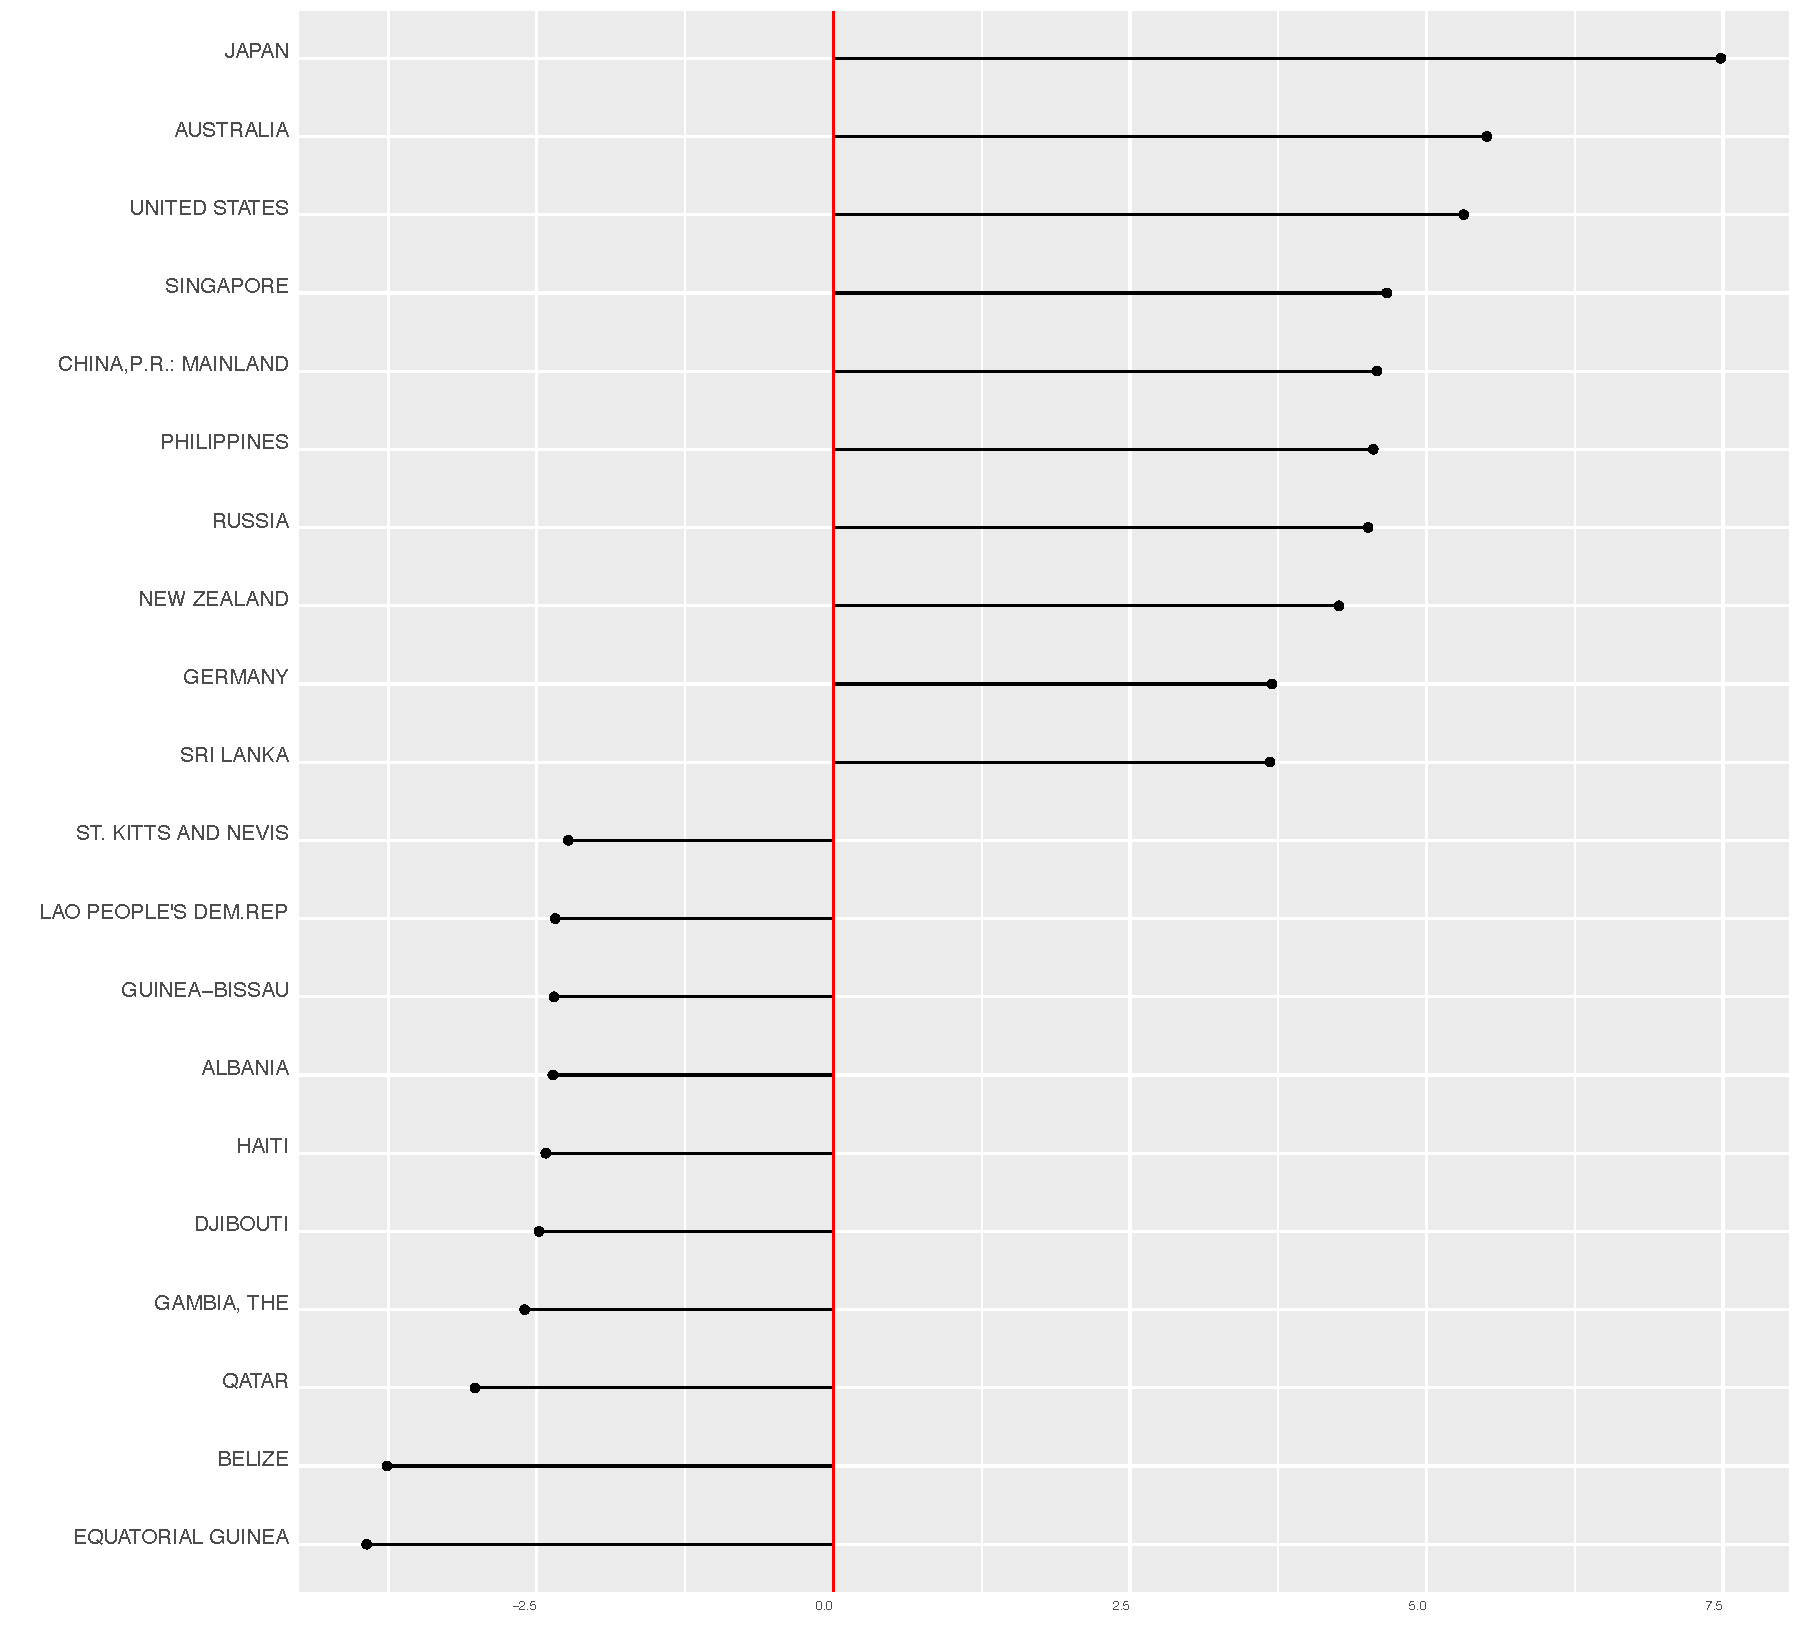
\includegraphics[width=65mm]{ABplot_rose_top10.pdf}}
%\subfigure[Receiver Random Effects]{\label{fig:rosereceive}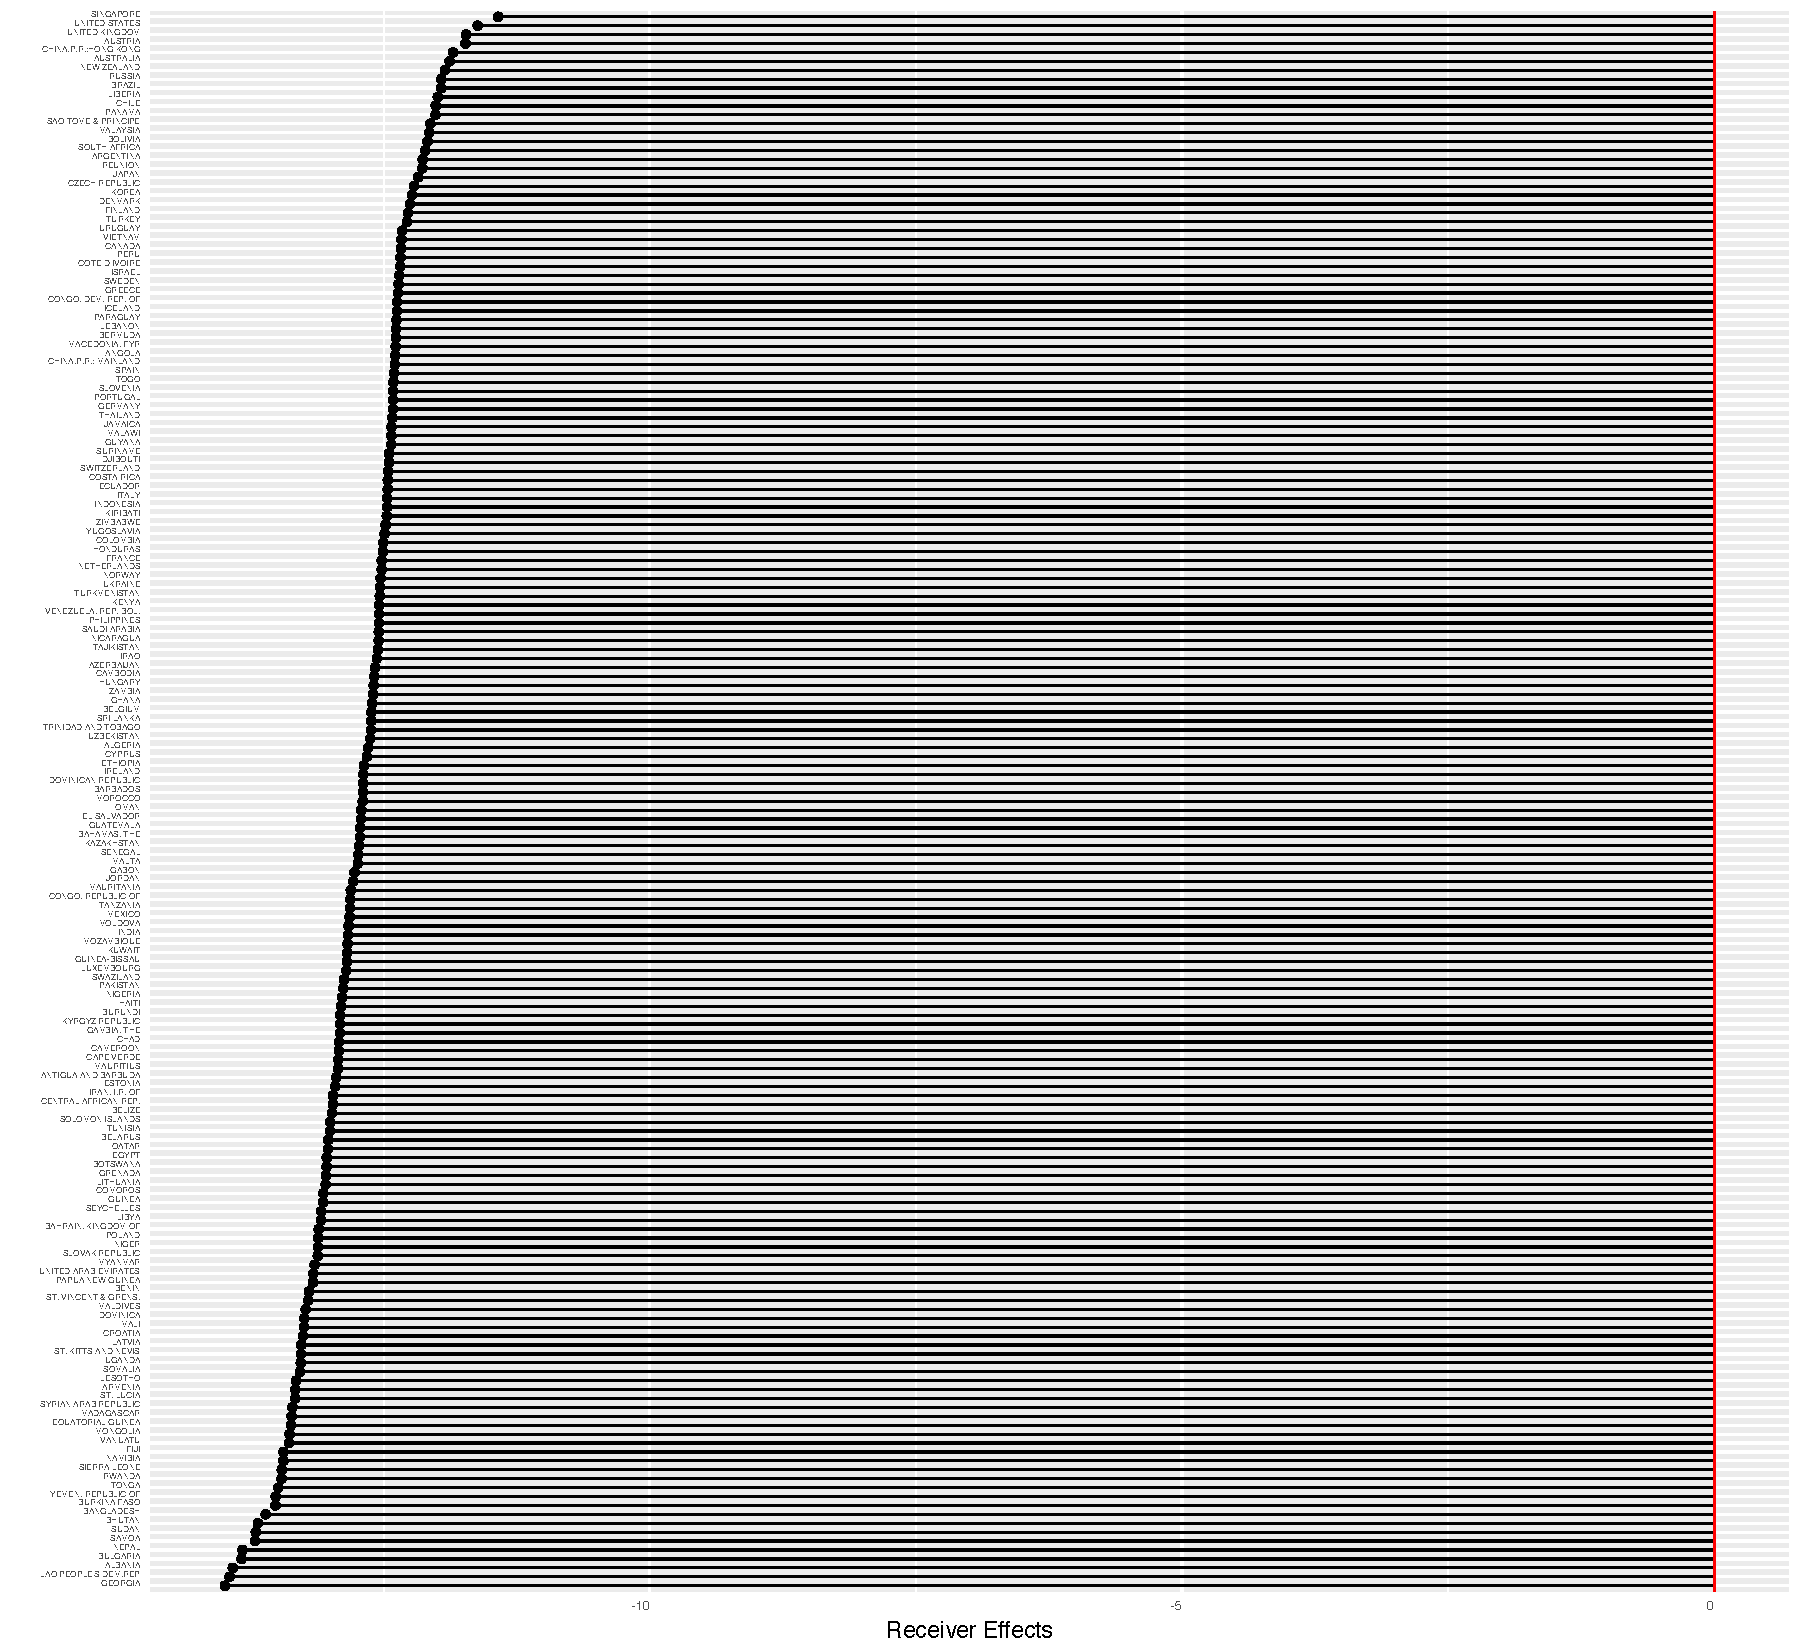
\includegraphics[width=65mm]{ABplot_receiver_rose.pdf}}
%\caption{Sender and receiver random effects for AME estimation of Rose (2004).}
%\label{fig:rosesr}
%\end{figure}

\newpage
\subsection{Replication of McDonald (2004)}

\citet{mcdonald:2004} studies whether trade promotes peace between nations. He observes that knowledge about the link between conflict and trade is indeterminate in the field of international relations, noting that competing explanations persist. He calls for more precise empirical tests.  Importantly, \citet{mcdonald:2004} includes the interdependence argument---that interdependence between states ``makes conflict less likely because of its efficiency over conquest in acquiring resources\ldots (547)'' in his overview of underdeveloped hypotheses. 

Accordingly, the primary contribution of the study is to provide evidence challenging the generalized linkage between peace and trade and to offer a new measurement of the key independent variable, trade. To do so, \citet{mcdonald:2004} refines the trade variable, arguing that \textit{free} trade, rather than trade alone, reduces the likelihood of conflict between states. His key hypothesis that greater levels of protection increase the probability of interstate conflict, an argument that builds on the work of classic liberalism and connects free trade to the power of domestic audiences. \citet{mcdonald:2004} measures free trade in two ways. The first  captures the idea that larger protected sectors generate greater societal pressures resulting in  pockets of support for war. This protection variable measures the proportion of customs revenue divided by total imports in the state that possesses the greater such ratio in each dyad. This measure captures the score of the state in the dyad that possesses higher barriers to trade (560). \citet{mcdonald:2004} also includes a measure of economic integration  calculated as ``the lower proportion of total dyadic trade (imports plus exports) divided by state i's GDP or total dyadic trade divided by state j's GDP.'' (560). Finally, the binary, dependent variable is the onset of a new militarized interstate dispute within a given dyad. \citet{mcdonald:2004} employs logistic regression to examine the putative statistical significance of these variables. The models include a spline correction for time-series data as well as robust standard errors clustered on each dyad.

% TO DO: include discussion and analysis of different K's in appendix (for M cD)
\begin{figure}
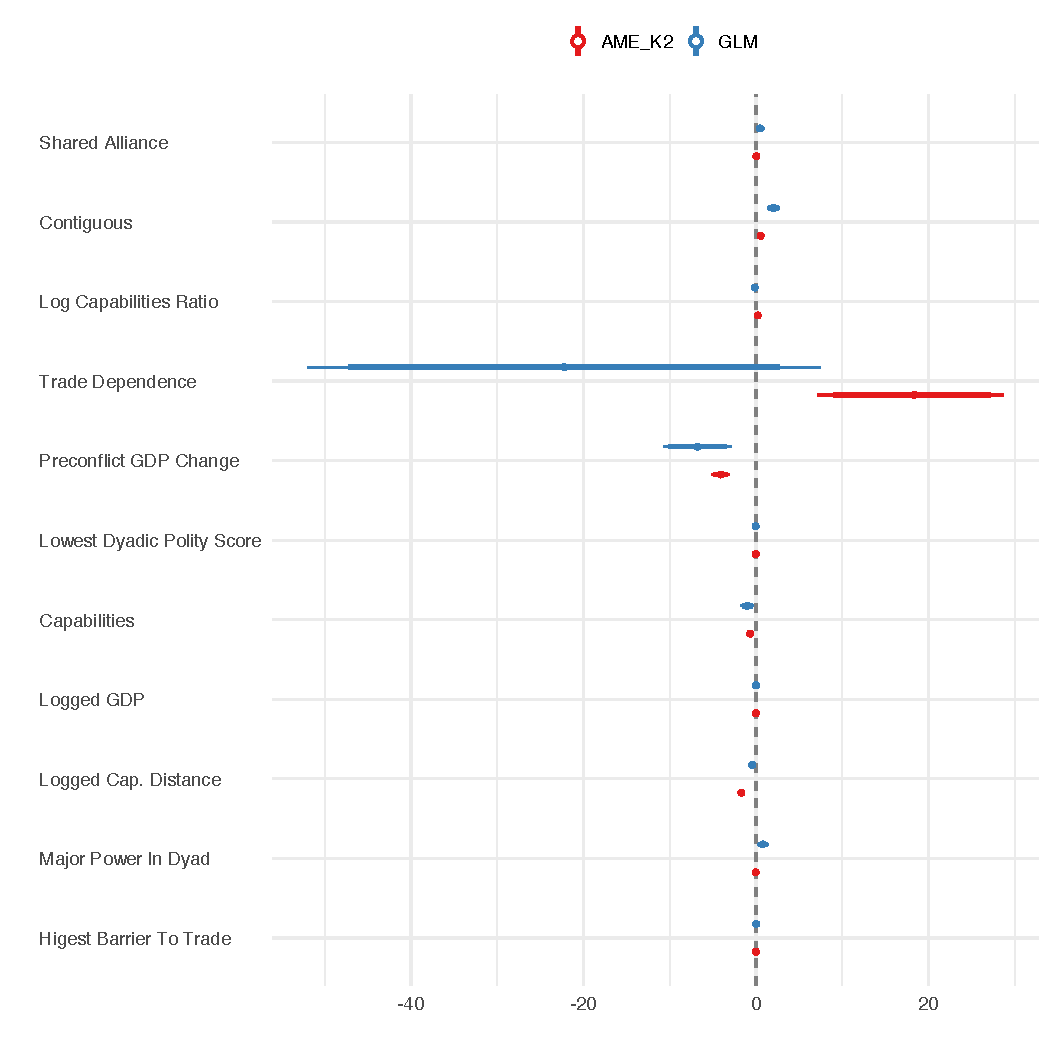
\includegraphics[width=\textwidth]{McDonald_coefs.pdf}
\caption{\label{fig:mcdCoefs}Coefficient plot of McDonald (2004)'s original model (blue) compared to AME model (red).}
\end{figure}

\begin{figure}
\centering   
\subfigure[AUC]{\label{fig:mcDauc}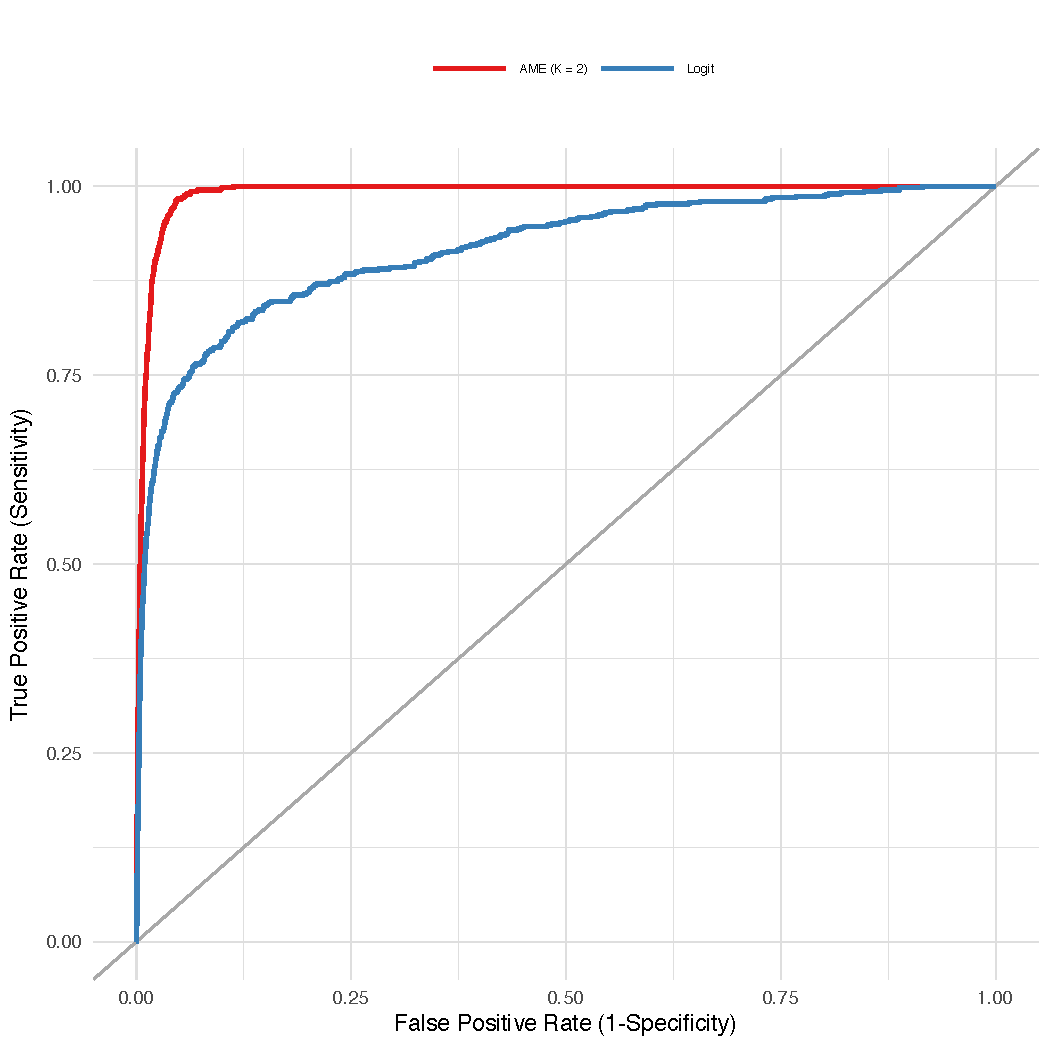
\includegraphics[width=65mm]{McDonald_auc_outsamp.pdf}}
\subfigure[Precision and Recall]{\label{fig:mcDpr}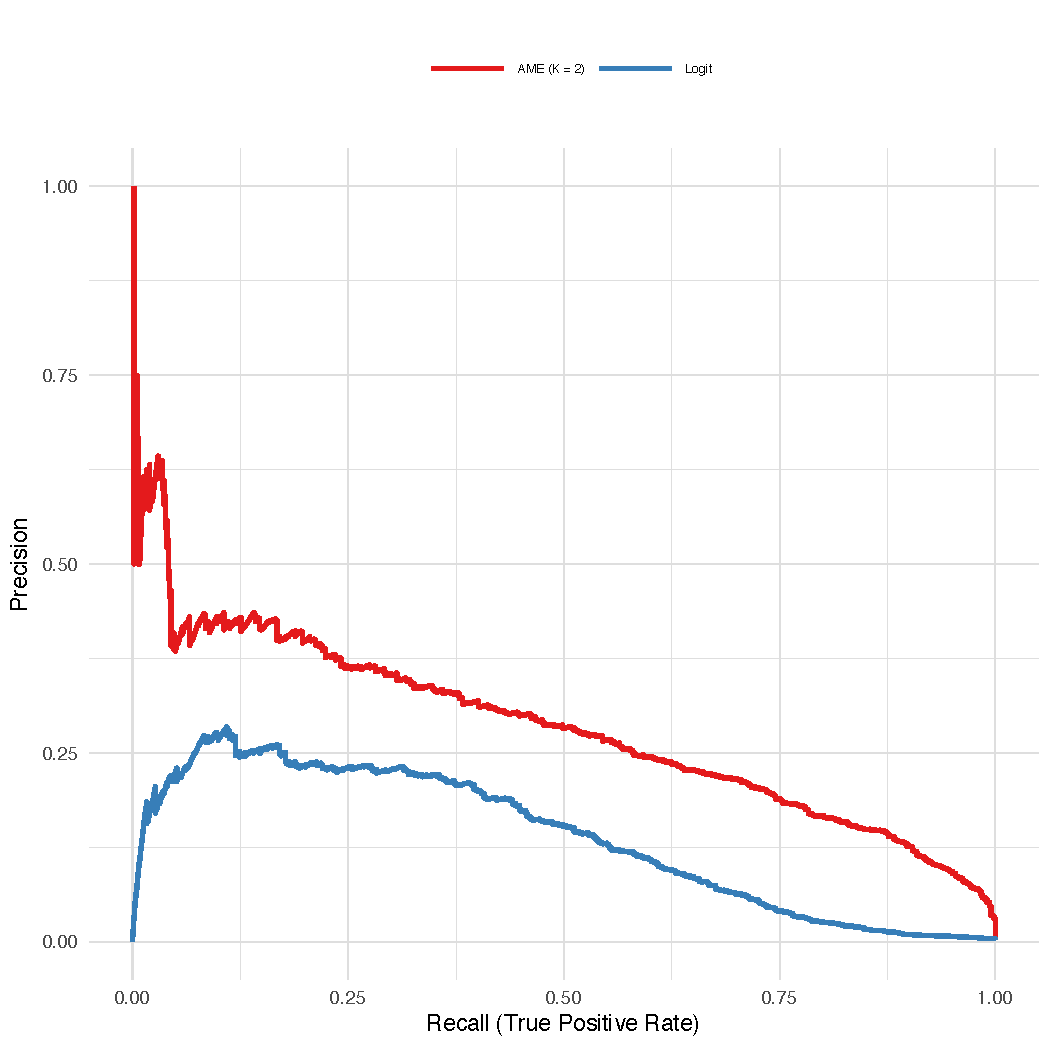
\includegraphics[width=65mm]{McDonald_pr_outsamp.pdf}}
\caption{\label{fig:mcdall} Assessments of out-of-sample predictive performance for McDonald (2004) using ROC curves and PR curves.}
\end{figure}

% TO DO: fix bib

Our replication reveals that trade relations are highly interdependent and exhibit important patterns of transitivity.  Or, in other words, if countries {i} and {j} are highly dependent and countries {j} and {k} are also highly dependent, then we are likely to observe high dependency between countries {i} and {k}. Our findings support those of Traag and Lupu (2013) which argue that indirect trade relations reduce the probability of conflict. This indicates that conflict is less likely between members of a trade community. Once we control for these dependencies, we can more clearly interpret the positive link between trade and conflict. Figure~\ref{fig:mcdCoefs} shows the coefficients for both the original and replicated model and Figure~\ref{fig:mcdall} demonstrates the predictive performance of each model. Figure ~\ref{fig:mcdcirc} represents the multiplicative effects of the model. This plot enables us to consider actors with similar sending and receiving patterns resulting from stochastic equivalence and homophily. In the upper arch for senders, there is a clear clustering of United States' allies (the United Kingdom, Netherlands, and Japan). We also observe an African cluster in the top right segment for receivers (Egypt, Niger, and Zambia for example). These countries both trade amongst themselves and have similar conflict behavior -- stochastic equivalence is present among the first group, homophily among the second -- and so once we account for these clusters using the multiplicative effects, the residual effect of trade actually increases the likelihood of conflict.

\begin{figure}
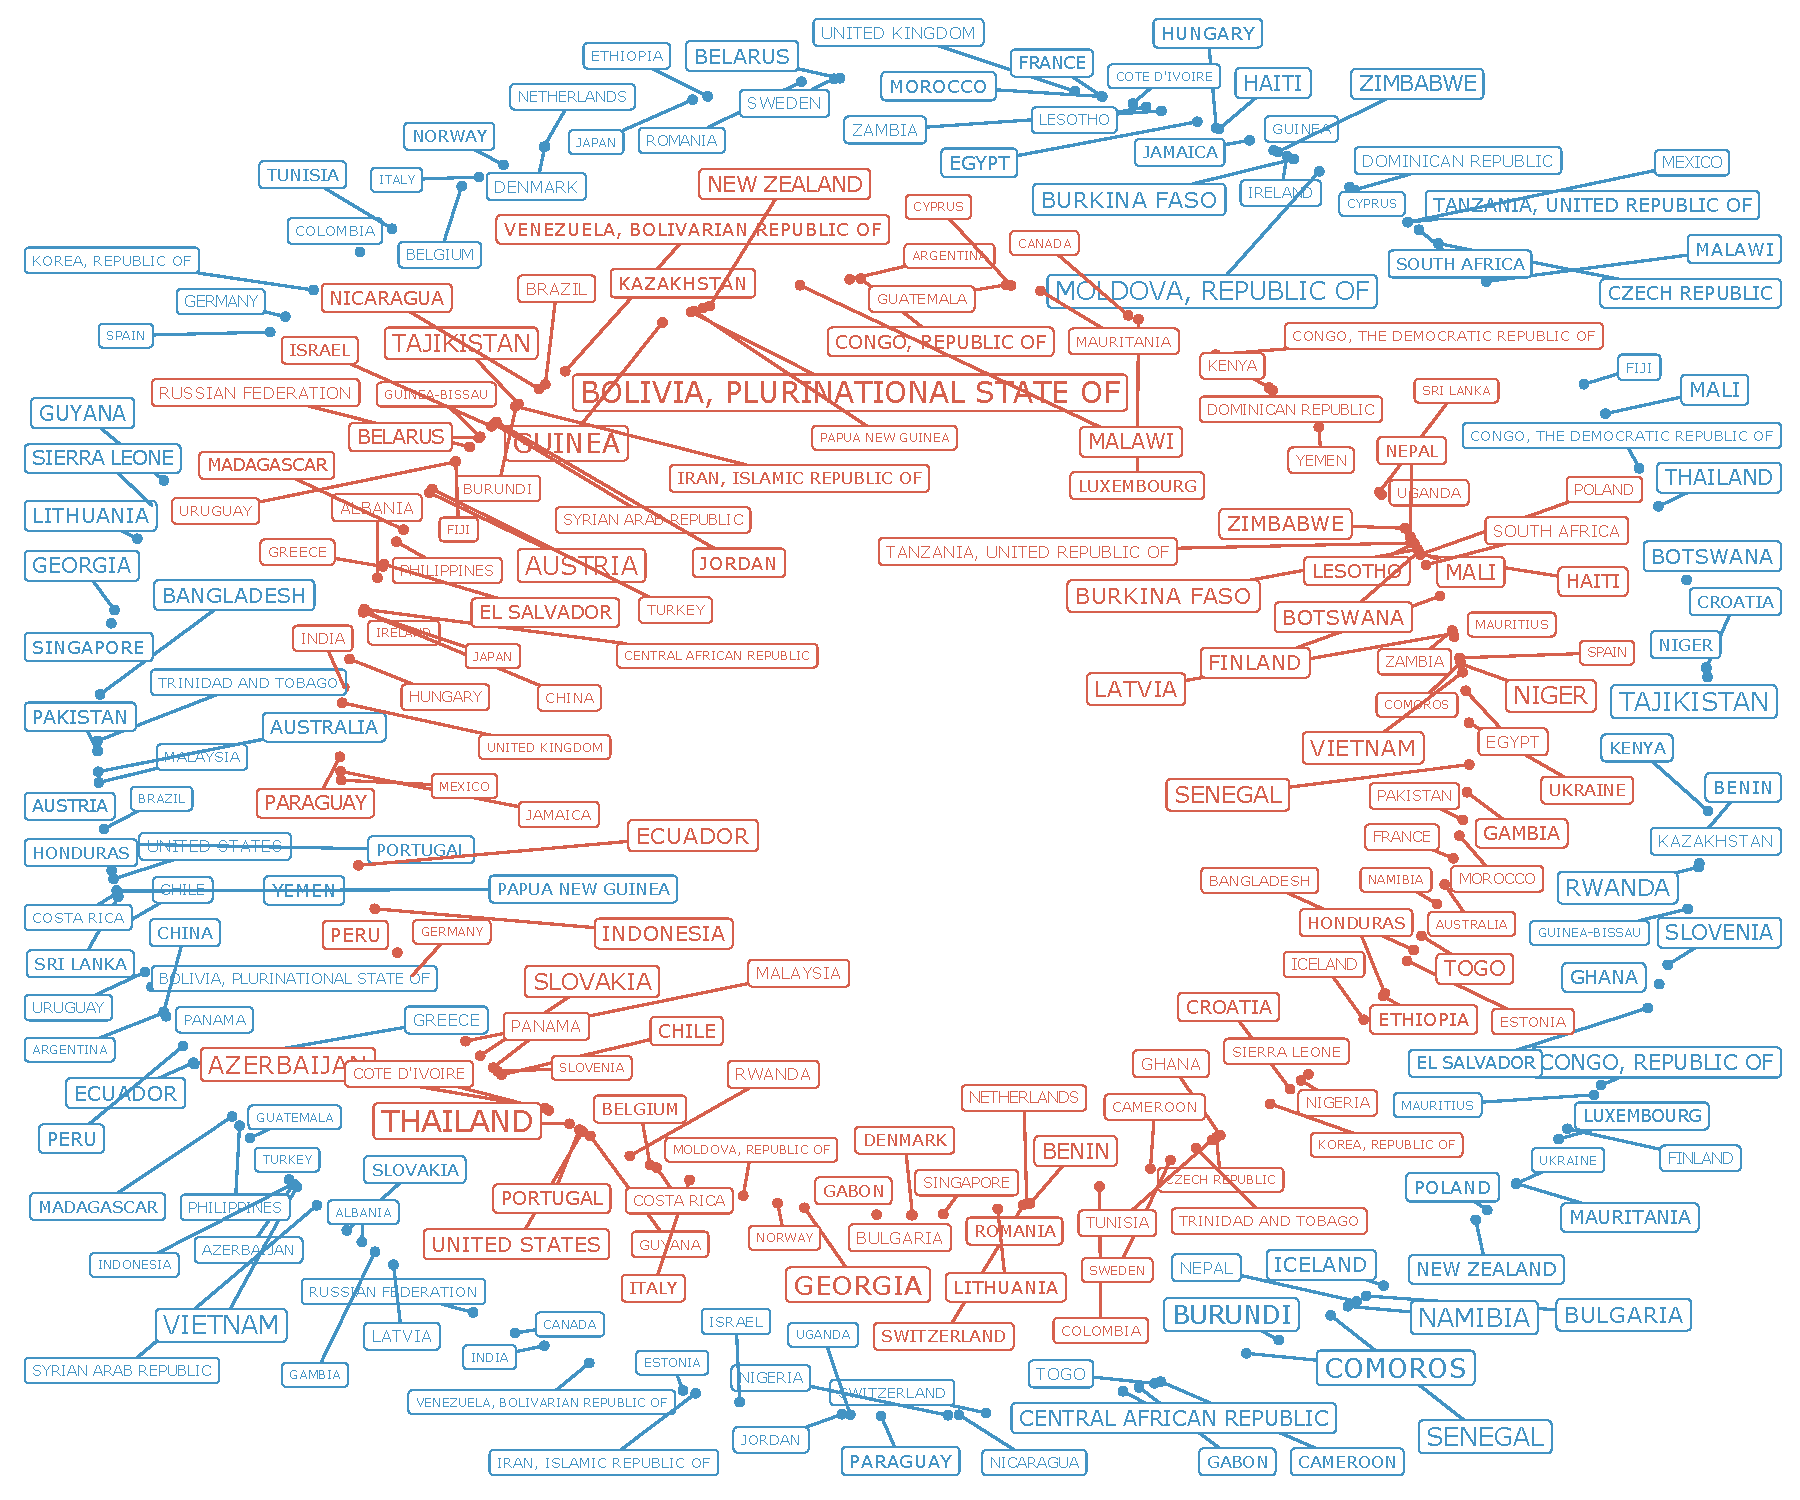
\includegraphics[width=\textwidth]{mcdonaldcirc.pdf}
\caption{\label{fig:mcdcirc} Visualization of multiplicative effects. Blue represents groups with common sending patterns and red represents groups with common receiving patterns.}
\end{figure}

\subsection{Replication of Gibler (2017)}

% We chose this article because it is published in 2017, demonstrating that the concern with interdependence continues to the present and because it was published in the so-called flagship journal of political science, \textit{The American Political Science Review.} It examines the link between dyadic capability differences and international conflict in terms of how and when states became independent members of the international system.  It assumes that membership in the international system---defined in typical ways---has a substantial influence on capabilities. In the same way that capabilities don't seem to vary enormously over time, at least comparatively, states become independent in a particular location, clustered with surrounding states. Neither does this change much over time. Gibler shows that the long-standing relationship between the relative parity of capabilities and initiation of international conflict is almost completely mediated by the initial conditions for the members of the dyad when they joined the international system as sovereign members. This finding calls into question many IR theories about the role of balance in terms of generating international conflict \citep{organski:1958}.

The replications we have undertaken are all from articles over the past fifteen years.  A more recent example is \citet{gibler:2017} which examines the onset of militarized disputes using capabilities, joint democracy, alliances, and power parity in a undirected dyadic study using logistic regression and dyad clustered standard errors.   In addition to this, Gibler shows that the long-standing relationship between the relative parity of capabilities and initiation of international conflict is almost completely mediated by the initial conditions for the members of the dyad when they joined the international system as sovereign members. This finding calls into question many IR theories about the role of balance in terms of generating international conflict \citep{organski:1958}.

\begin{table}
\begin{center}
\caption{Comparison of Gibler (2017) Model 6 results with AME results. This was run over a chain of $10,000$ iterations.  \label{tab:gibme}}
\begin{tabular}{lrr} \toprule
& \multicolumn{2}{c}{$\hat{\beta}$ Estimates}\\ \cmidrule{2-3}
Variable & \texttt{logit} & \texttt{amen} \\ \midrule
Allied & 0.142&  0.023 \\
Joint Democracy &\bf -0.507&  0.045 \\
Peace Years \bf &-0.260& \bf -0.060 \\
Spline 1 &\bf -0.001& \bf 0.00 \\
Spline 2&\bf -0.000& \bf 0.00\\
Spline 3 &-0.000& \bf 0.00\\ 
Contiguity &\bf 2.412& \bf 0.640 \\
Parity &0.075&  -0.013 \\
Parity at entry year&\bf 0.868&  0.002 \\ 
Rivalry &\bf 2.031&\bf 0.721\\ 
Constant &\bf -5.526 & \bf  -2.581\\ \bottomrule
\end{tabular}\\
\end{center}
{\bf Note}: {\bf Bold} indicates conventional statistical significance at $p < 0.05$ or less in Gibler (2017). For comparative purposes, only, we have employed the same criterion to the results from the \texttt{amen} estimation.
\end{table}

We re-estimated model 6 from Table 6 (2017,34). The results are presented in Table~\ref{tab:gibme} in order to facilitate explicit comparison.
The results obtained with \texttt{amen} stand in stark contrast to those found with a logistic regression (with dyad clustered, robust standard errors).  Most importantly, the primary variable from the Gibler study, parity of the members of a dyad at the year in which they entered the international system, is shown to be unimportant in the amen results.  Not only is the value of the this parameter small, but it has a very large relative standard error, over a magnitude larger than the parameter itself ($z= 0.038$). In addition, joint democracy follows the same pattern of importance in the logistic results, but this disappears once interdependencies are modeled.  As might be expected the strong geographic clustering in the original study is about one-quarter as strong in the \texttt{amen} estimations. Similarly, rivalry coefficients are about one-third the size in the \texttt{amen} formulation, but a great deal more precisely measured ($z=18.116$). 

Beyond more informative fixed effect coefficients, the \texttt{amen} approach also provides information about the interdependencies that were modeled. The most pertinent of these may be the dyadic and triadic dependencies which are presented in Figure~\ref{fig:gibler:dyadtriad}, which further reveal that the assumption of independence among the dyadic data in this study can be strongly rejected. Perhaps most importantly, the main substantive conclusions of the 2017 Gibler study do not seem warranted from the perspective of the results obtained with the \texttt{amen} estimation that explicitly models \first- \second-, and \third-order interdependencies. Not only do the estimated coefficients tell a different story, but the assumptions under which the original results would hold are shown to be violated by the data.

% sd.rowmean sd.colmean   dyad.dep  triad.dep 
% 0.03210221 0.03210221 0.99362646 0.00130249 
\begin{figure}
\caption{\label{fig:gibler:dyadtriad} The left panel is  a plot of the dyadic dependencies in the Gibler model 6; the right panel shows the triad dependencies.  Note that the red line represents the null hypothesis of no dependencies, indicating that the standard logistic approach is far from what is uncovered with this analysis. }
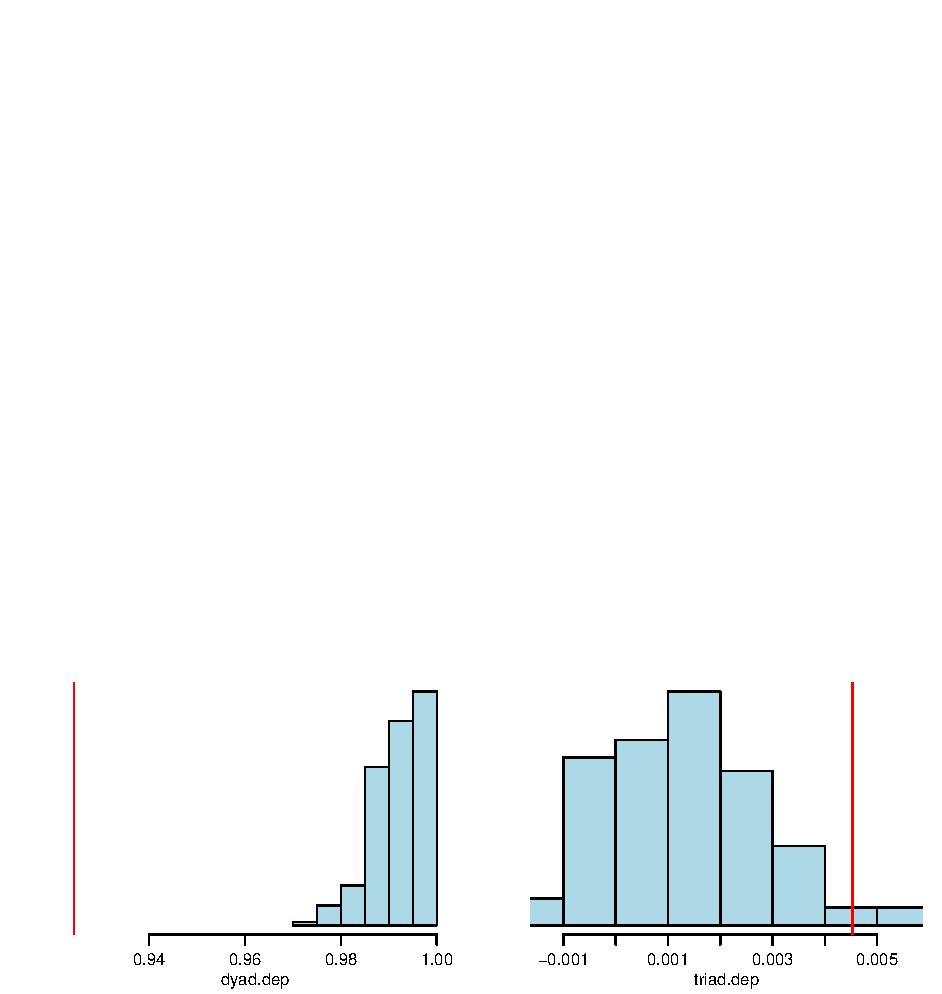
\includegraphics[width=\textwidth]{netplots}
\end{figure}
\FloatBarrier
